\documentclass[a4paper, 12pt]{article}
\usepackage{tabularx}
\usepackage{amsmath}
\usepackage{graphicx}
\usepackage[margin=1in,letterpaper]{geometry}
\usepackage{cite}
\usepackage[final]{hyperref}
\hypersetup{
	colorlinks=true,
	linkcolor=blue,
	citecolor=blue,
	filecolor=magenta,
	urlcolor=blue
}

\begin{document}

\title{CENG532 - Distributed Computing Systems Project Report}
\author{Burak Hocaoglu 2035988, M. Rasit Ozdemir 1942606}
\date{\today}
\maketitle

\begin{abstract}
In this experiment we studied the problem of establishing coordination and consensus over a P2P network topology with each node operating asynchronously. By nature, solving this problem is impossible, but under a set of conditions, this problem cen become tractable. Based on this idea, in this study, we have designed a protocol combining several aspects of already existing studies and shown the experimental results in a simulated environment called \textbf{Mininet} with its Python API. For the whole source code, log history and simulation results refer to the \href{https://github.com/burakceng/CENG532-DistributedComputing-Project.git}{Github repo}.
\end{abstract}

\section{Introduction}

The problem of establishing coordination and consensus on a network with asynchronously operating nodes is considered to be impossible to solve. Coordination and consensus indicates data consistency and time synchronization issues. For example, when multiple nodes are responsible for storage and update of a specific data (i.e. replicated data) or database management where transactions can lead to \textit{commit} procedures, data consistency is to be provided to prevent unexpected behaviour from happenning. Usually commit procedures contain timestamps to put requests that will change the data in timestamp order and to achieve consistency each replica of the data is updated with respect to this timestamp order. Many studies have been conducted in order to solve this problem; however, this problem is considered to be impossible to solve by nature and can only be solved as long as some pre-determined conditions are satisfied. These conditions usually involve global time synchronization, probability of occurrence of several factors related to the underlying network, i.e. packet losses, reordering, noise and error issues etc.

In this study, we will give our reliable multicast protocol design with experimental results under the conditions that we assumed. In Section 2, we will mention which assumptions are made as for how the experiments are conducted and what our design requires to operate regarding the Mininet environment. Mininet is a simulation environment which is used for simulating distributed systems by mapping each working procedure/process to an actual Operating System process. In Section 3, we describe the execution principle of our design, what kind of packets are exchanged in order to achieve the purpose of establishing consensus with preserving total-order property. In Section 4, we present the rough algorithm in pseudocode form. Finally, in Section 5, we present the performance analysis of our design with what type of experiments are used to gather data.

\section{Assumptions on the Protocol}
As stated before, to be able to solve a problem that is impossible to solve, we present a set of assumptions/conditions to work under so that the solution space becomes restricted enough to find a feasible methodology or to make the problem tractable. The following are the assumptions for this protocol design with some of them are included for the sake of easy experimenting:
\begin{itemize}
    \item Since the experiment environment utilizes a single hardware, all processes will share the same CPU clocks; hence, same global time reference. Although the processes can be distributed over the multiple cores of the CPU integrated to the hardware of interest, the clock diferences between each core will have negligible difference. Therefore, we assume that all processes/nodes in our network topology are inherently synchronized in terms of global time reference. One can claim that if global synchronization is guaranteed, the problem is already solved; however, this claim does not include the fact that Mininet works on a single hardware in our discussion, where any context switch between processes will result in that only one of the nodes will be using the CPU and the others will be asleep, which will introduce packet losses indirectly (even though experimenter did not add any simulated loss factor to a link) since sleeping nodes are not able to poll their queues whether a packet has arrived or not. This also indirectly results in re-ordered packets.
    \item Each node in the topology will have the same amount of packets to multicast. This is for the sake of easier experimenting. However, in order to introduce stochasticity in terms of which packets will be multicasted by which node, each experiment will start with nodes having a set of random sequence numbers from a range between minimum and maximum possible number. In other words, between two experiments a node may not multicast same sequence numbers, but regardless of the randomness, the amount of packets will be equal for each node in the network.
    \item We will assume that all nodes will know the nodes in the network, but this assumption does not guarantee the availability of a node. In other words, each node will know the other members of the network, but the node may be crashed/died or there may be a link failure that might lead the node to deduce a similar situation.
    \item As for bit errors in the messages, we will assume there will not be errors, since Mininet environment does not provide a way to introduce a recoverable noise mechanisms.
\end{itemize}

\section{Execution Principle of the Protocol}

\subsection{The Topology and Configuration}
In physical sense, the topology is a star network; however, the experiments will assume a different logical topology based on group size. In our experiments we made use of a topology with 5 nodes and a switch in the center in Mininet environment. \ref{mininet}

\begin{figure}[h]
\centering
   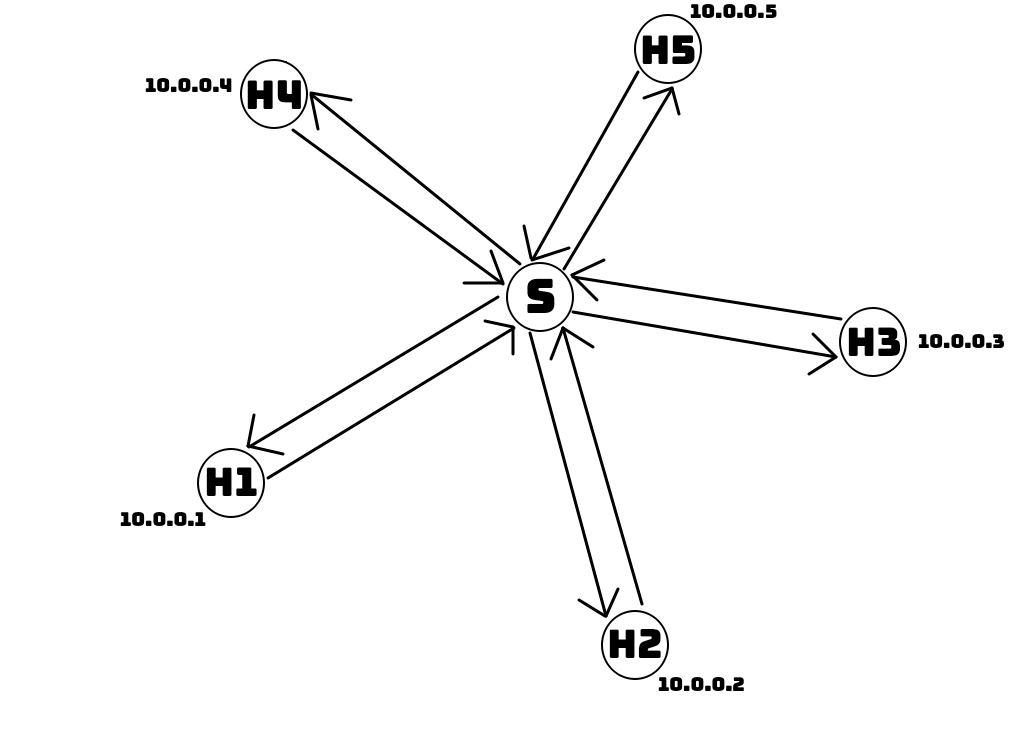
\includegraphics[scale=0.45]{mininet_topology.png}
   \caption{Mininet physical network topology}
   \label{mininet}
\end{figure}

The first logical network we designed will form a Chord-like topology without making use of communication mechanism of Chord. Every node has 2 nodes as receiver group and sequence numbers of these nodes are randomly generated by the configuration initialization script. \ref{chord}


\begin{figure}[h]
\centering
   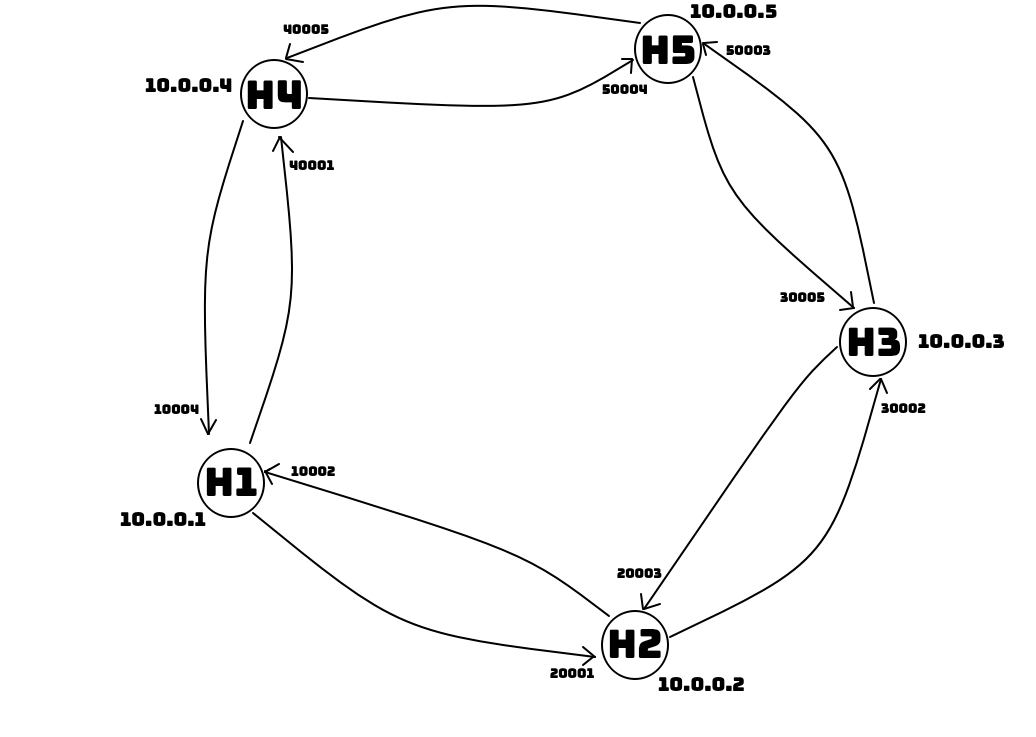
\includegraphics[scale=0.50]{conf2.png}
   \caption{First logical network topology (Chord-like)}
   \label{chord}
\end{figure}


The second logical network we designed will form a semi-star topology. Almost every node has 3 nodes in receiver group except one node that has 4 nodes in its receiver group. \ref{semi-star}


\begin{figure}[h]
\centering
   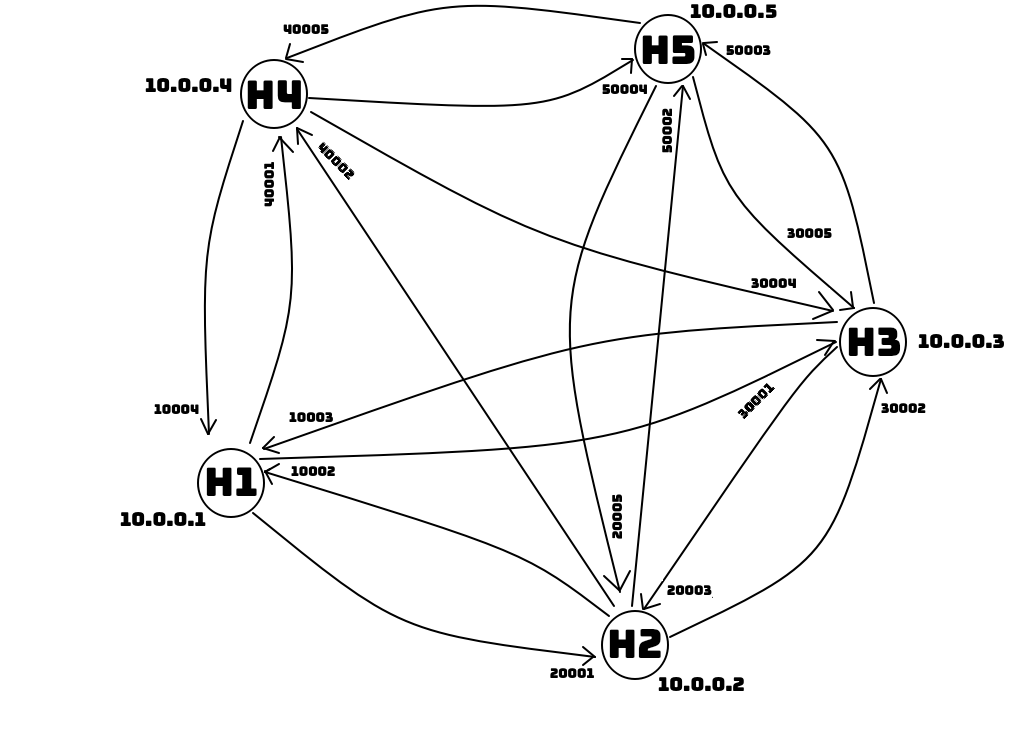
\includegraphics[scale=0.50]{conf3.png}
   \caption{Second logical network topology (semi-star)}
   \label{semi-star}
\end{figure}

The third logical network we designed will form a full-star topology. Every node has other nodes in its receiver group.

For the sake of simplicity, the naming convention of the nodes in the network is set as \textit{Hi} for the \textit{i}th node, e.g. \textit{H4} for the fourth node. In addition, each node will have a list of sequence numbers of equal length, where the numbers are randomly sampled from a range of numbers without replacement. For example, a topology of 3 nodes is given and an experiment will consis of 6 packets that are exchanged over the network, i.e. each node will have $\frac{6}{3}=2$ packets to multicast to its neighbours. The following is a valid example of how sequence numbers can be shared randomly:
\begin{itemize}
    \item Sequence number range: $\{1, 2, 3, 4, 5, 6\}$,
    \item Node H1 has $ \{1, 6\}$,
    \item Node H2 has $ \{2, 5\}$,
    \item Node H3 has $ \{3, 4\}$.
\end{itemize}

\subsection{Node Structure}
Each node fundamentally has the following:
\begin{itemize}
    \item \textbf{Name:} The name of the node in the network
    \item \textbf{Sequence List:} A list of sequence numbers that the node will be multicasting
    \item \textbf{Interfaces:} A list of the neihgbours' names mapped to the particular interface for communication
    \item \textbf{Sockets:} A mapping of sockets to the interfaces to communicate
    \item \textbf{Clock:} The vector clock from the node's point of view
    \item \textbf{Queue:} The queue of incoming packets/messages that are to be \textit{delivered} to the node's application layer.
    \item \textbf{ACK Table:} The table of neighbours mapped to the state of whether they have received the multicasted packet of interest
    \item \textbf{Deliver ACK Table:} Same as the ACK table but works for \textit{delivery} process, i.e. processing the packet in the application layer.
\end{itemize}
In addition to the above, all nodes have necessary data structures for synchronization of its threads that are used for each communication link they have.

\subsection{Packet Content}
\begin{itemize}
    \item \textbf{Type:} The type of the packet, there are 4 types:
    \begin{itemize}
        \item \textit{Multicast:} 1
        \item \textit{Multicast ACK:} 2
        \item \textit{Deliver:} 4
        \item \textit{Deliver ACK:} 8
    \end{itemize}
    \item \textbf{Source:} The name of the node that initiates the multicast
    \item \textbf{Destination:} The list of nodes who constitute receiver group
    \item \textbf{SequenceNumber:} Sequence number of the packet
    \item \textbf{LocalOrder:} The index - starts from 0 - of the sequence number in the node's sequence number list
    \item \textbf{Timestamp:} Global timestamp with respect to the CPU clock
    \item \textbf{Vector:} Logical clock of the sender node (advanced before initiating a multicast)
\end{itemize}

% MIGHT AS WELL ADD A DIAGRAM HERE

\subsection{Execution Principle}
Under normal circumstances, each node periodically sends multicast messages with its logical clock for synchronization to its all \textit{logical} neighbours, i.e. with respect to the logical topology. If the receiving group has successfully received the message without any errors, then each node in that group will send a Multicast ACK message to indicate that it is ready to \textit{deliver} the message. If the multicast initiator receive a Multicast ACK and the sequence numbers match, then the sender sets the corresponding neighbour entry of its ACK table to \textbf{True}. When all entries of that table is set to true, then the initiator can multicast a \textit{Delivery} request to the receiving group of interest. Upon receiving the delivery request, the receiving group will process the packet received previously via multicast and update their logical clocks accordingly. After having updated, each node in the receiving group will send a \textit{Deliver ACK} message to the initiator indicating that it is ready to receive the next regular message, i.e. packet with type 1. Similar to multicast phase, the initiator will make sure that it received a Deliver ACK from all members of the receiving group fo that particular message, which involves a Delivery ACK table working similarly.

In order to have high concurrency, our protocol imposes a relaxed sequential execution semantic, by letting each node multicast its messages asynchronously without waiting for a consensus for that particular message. However, to achieve \textit{atomic broadcast} properties, establishing a consensus on the order of message deliveries is what aimed by our protocol. In our protocol, the main aim is to preserve the order. To achieve this under the assumptions we made, we introduce a \textbf{local order} proposed by every node only for their messages. Every node adds this data to the corresponding fields of their packets to inform the receiving group if there wwas supposedto be another message before the one being multicasted (this idea is inspired from the \textit{soft-sync} concept of \cite{FastCast}, where the group has a local synchronization mechanism involving the multicast order of the message and the global timestamp). We propose this idea, since we aim to increase CPU utilization. If we did not introduce this data, the nodes may have to wait until at least one message exists in each of their receiving queues. Following the idea of null messages being multicasted repeatedly until the process is ready to process a message in the queue from \cite{CMB}, we repeatedly send the messages required to be delivered to the neighbouring nodes; however, these are not null messages in terms of content, but similar to null messages in the sense of not being delivered (e.g. ACK feedbacks and Delivery Requests). Back to the local order data, it is used in queue ordering with the timestamp of messages obtained from global clock. Each receiving queue is connected to a priority queue (i.e. a min-heap) which prioritizes the messages sent earliest and with the lowest local order (in terms of numerical value, since it indicates index).

When a non-zero packet loss probability is introduced to the links, the protocol imposes \textbf{All-or-None} semantics, i.e. the initiator node will make sure that all of the nodes in the receiving group related to the multicast context have received the message multicasted. Each socket associated with each node has a timeout value that is 4 times (experimental value) of its regular period. If a multicast ACK message is lost, then timeout interrupt will start a re-transmission procedure. In other words, a timeout mechanism is used for packet loss detection. When one considers a node/link failure, since under these situations a node cannot make sure that one of its messages would arrive the destination, i.e. packet loss, our protocol treats those phenomena as packet losses as well. The timeout check starts right after a node sends a message through one of its sockets and the timeout for all sockets of a node and across all nodes are equal.

The feedback mechanism is simply built on ACK type packets with having the same content as the packet which is supposed to be ACKed, but having certain fields changed for obvious reasons, e.g. source, type and timestamp fields. The feedbacks are handled depending on what \textit{state} that the node is in. There are 3 states in operation: \textbf{MCAST}, which sets the node behaviour to only accept/process (not actually deliver, some of the messages are to establish consensus, they are not meant to be delivered) the messages which are either regular multicasts or multicast ACKs; \textbf{DCAST}, similar to the previous with the message types of interest are deliver requests and deliver ACKs; \textbf{FINISH}, which indicates that the node has no messages left to be multicasted and works for establishing consensus.

As for the existence of the nodes in the network, i.e. detecting whether they have died or not, is integrated with the normal message exchange mechanism. As stated before, if a node/link failure has occurred, since this will lead to packet losses, the nodes will only deduce from timeout interrupts that packets are lost. Under such a circumstance, we did not introduce a separate mechanism to distinguish failure cases from regular packet losses; therefore, the nodes do not stop sending messages hoping that the receiver nodes will receive it eventually.

\begin{figure}[h]
\centering
   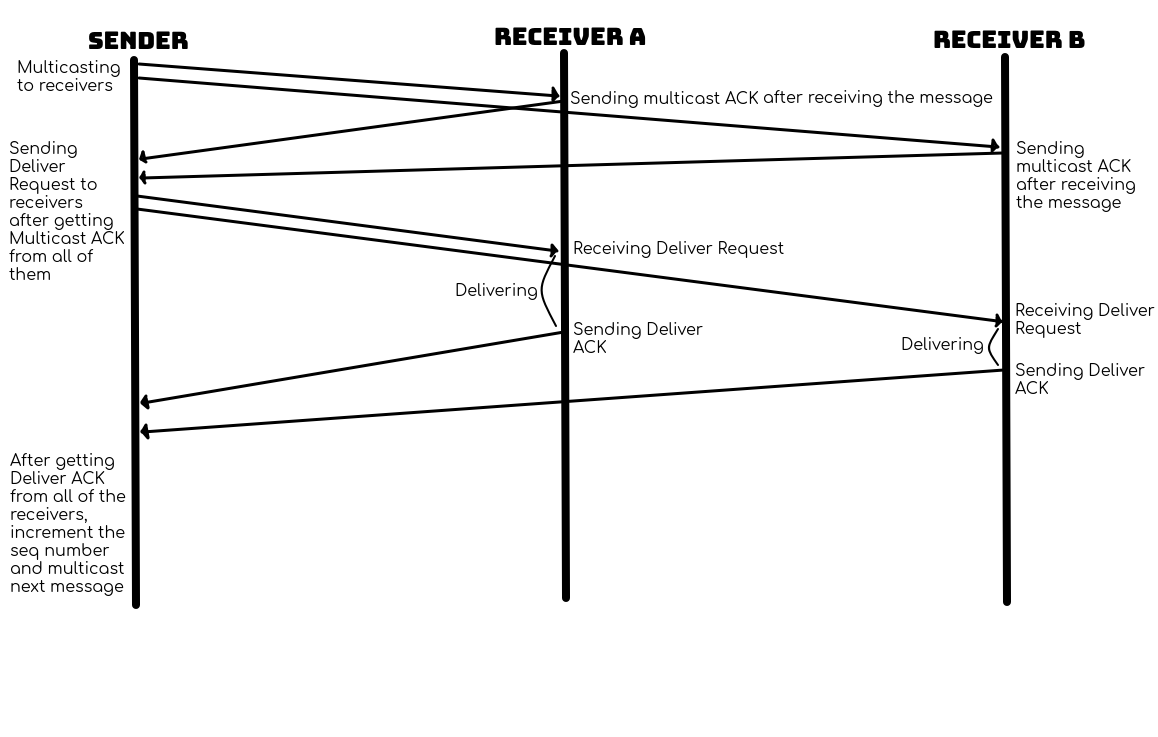
\includegraphics[scale=0.45]{diagram.png}
   \caption{Execution diagram}
   \label{diagram}
\end{figure}

\section{Algorithm}
The core of the algorithm is to both multicast messages to the network and listen to the network for incoming messages, asynchoronously, and advance execution only if the initiator node gives consent that the multicasted message is received/delivered by the destination group. This consensus is established by tracking the state of 2 lookup tables, one for multicast ACKs and the other for delivery ACKs. The receiver group is triggered only if the initiator is convinced that each member of the group has successfully sent a multicast ACK, i.e. all entries of multicast ACK lookup table is set to True. Then, delivery phase starts, and a similar procedure is applied. The only difference is the lookup table, which is utilized for tracking delivery consensus.

If the nodes receive a message which is already delivered by a member of the destination group, that member drops the packet immediately and sends an ACK message suitable to the type of the received packet, i.e. if type 1 is received, then a multicast ACK is sent; if type 4 is received, then a delivery ACK is sent. Even though packet losses occur, since our algorithm needs a consensus of 2 phases, no node advances its execution in a way that may violate total-order property of atomic broadcast. Therefore, we satisfy \textbf{Agreement} property, when the nodes enter delivery phase, since \textit{Agreement} property does not care about when the packets are delivered as long as all members of the destination group delivers the same packet. As for \textbf{Validity} property, the basis is similar to what we have described for \textit{Agreement} property, but in addition to that, \textit{Validity} property requires reliability under packet loss situations. To satisfy that, we designed our algorithm to repetitively send required messages until necessary ACK feedbacks are collected to advance the execution to the next phase. The \textbf{Integrity} property is a bit easier to fullfill, since the algorithm forces the delivery process to work depending on the state of the queue, i.e. if its empty, otherwise, which messages are received etc.; therefore, if no message is multicasted to a node, that node will not initiate a delivery process. Finally, the satisfaction of \textbf{Total-Order} property is explained in detail in previous section, where we mention the execution principle of our algorithm.

\section{Performance Analysis}
In this section, we present our experiment methodology and the results of our algorithm design by observing the behaviour of several factors related to the physicality of the network topology. The experiment environment is chosen as the aforementioned Mininet, which works on a virtual machine and provides a distributed networking environment, where each node is constructed as an operating system process and refers to the CPU clock of the hardware on which the virtual machine is running. Specifically, we made use of Mininet's Python API for flexibility of simulation and statistical data collection. Each of our experiments are a 5-minute slice of execution with various simulation parameters. The parameters are selected as \textbf{group size} and \textbf{packet arrival rate $\lambda $}, while the performance metrics are \textbf{avg. stable delivery time}(in seconds) and \textbf{efficiency}(total number of bits per one useful bit).

To be able to differentiate the timing performance, we introduced deliberate delays when multicasting and delivering. When multicasting, each message is multicasted with $0.5$ seconds of delay between one another, whereas in delivery phase, there is a $1.0$ second of delay after delivering the message to the application layer. Under ideal circumstances, for our smallest network with 5 nodes and 2 packets to be multicasted per node with each node having a group size of 2. Since there are at least 4 messages needs to be exchanged (i.e. 4 types of messages), and for each message we will perform a similar process for each member in the destination group, we will have to exchange at least $2*5*2*4=80$ messages. When packet losses and context switches introduced (Mininet does not work on a separate hardware, but in a VM), this number obviously will increase. To simulate packet loss factor, we applied 10\% loss to each link in the Mininet simulated topology.

% Group Size vs Avg. Delivery Time
\begin{figure}[h]
\centering
   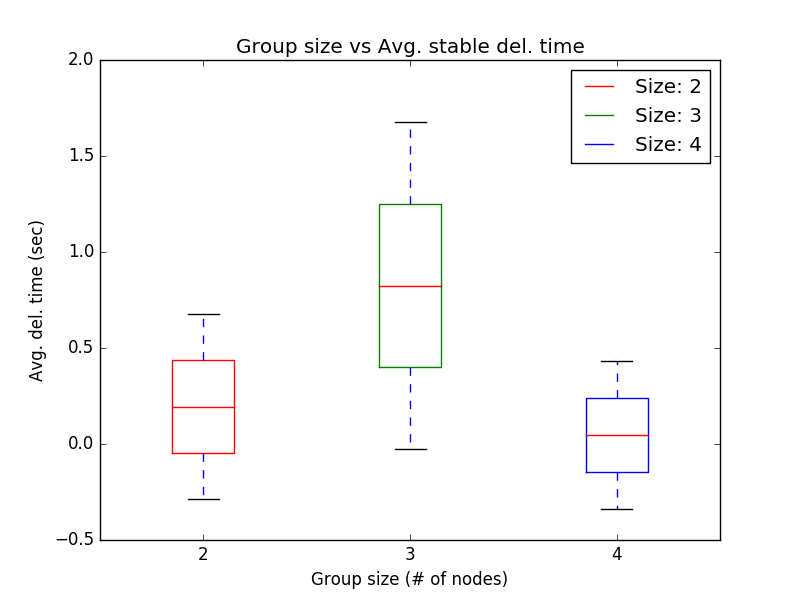
\includegraphics[scale=0.45]{GS_vs_AvgDT_Final.png}
   \caption{Group size vs. Avg. stable Delivery Time within 95\% CI}
   \label{gsvsavg}
\end{figure}

Observing Figure \ref{gsvsavg}, we can observe that since the delivery time is computed per packet delivered, even with the introduction of additional delays in multicast and delivery phases, the average timing is still below the aforementioned timeout limit, which is 4 times of the period of different multicast phases (for brevity, in all of our experiments we have set the period to $1.0$ second; hence, $4.0$ seconds of timeout duration). The issue with the case when group size is equal to 3 is that since we utilized a network with 5 nodes, if each node is to have 3 nodes as the destination group, one node will have to have either a 4-node group or 2-node group. We chose the 4-node for the last node making the message exchanges heavier compared to other regular nodes, which affected the overall average delivery performance considerably. The corresponsing means and standard deviations are $0.195 \pm 0.161$, $0.458 \pm 0.405$ and $0.147 \pm 0.095$ for group sizes 2, 3 and 4, respectively. The results have obtained from a total of 40 experiments for each group, having exchanged a total of 326034 packets, i.e. ~2717 packets per experiment.

% Lambda vs Avg. Delivery Time
\begin{figure}[h]
\centering
   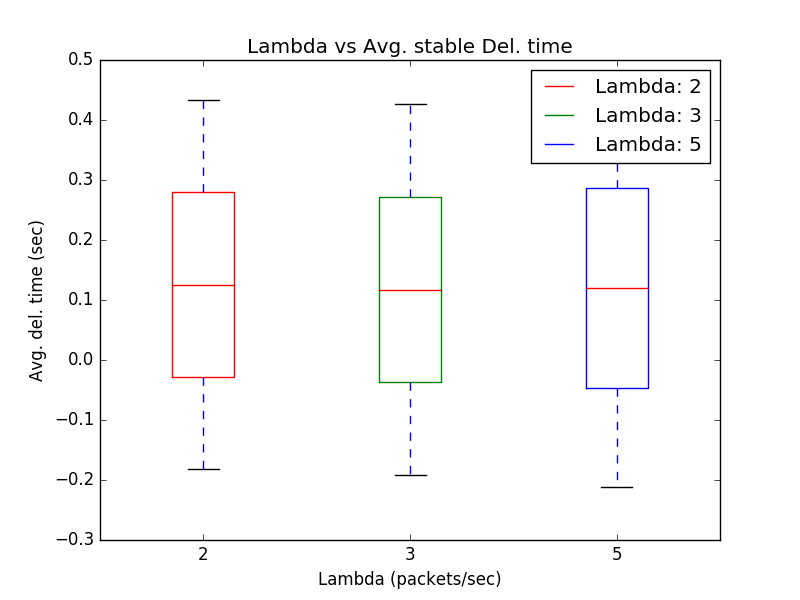
\includegraphics[scale=0.45]{Lambda_vs_AvgDT_Final.png}
   \caption{Lambda vs. Avg. stable Delivery Time within 95\% CI}
   \label{lbvsavg}
\end{figure}

The experiment whose results are associated with the Figure \ref{lbvsavg}, utilized a Poisson distribution with different lambda values chosen as 2, 3 and 5. Observing the results, the average stable delivery time is roughly the same across different lambda values, with the $\lambda = 2$ case being slightly higher overall because of a slightly higher standard deviation. For this experiment, the means and standard deviations are $0.126 \pm 0.102$, $0.117 \pm 0.103$ and $0.120 \pm 0.110$ for lambda values 2, 3 and 5, respectively. The total number of packets exchanged is 53207, having conducted 10 experiments per value, in one experiment an average of ~1774 packets have been exchanged.

% Group Size vs Efficiency
\begin{figure}[h]
\centering
   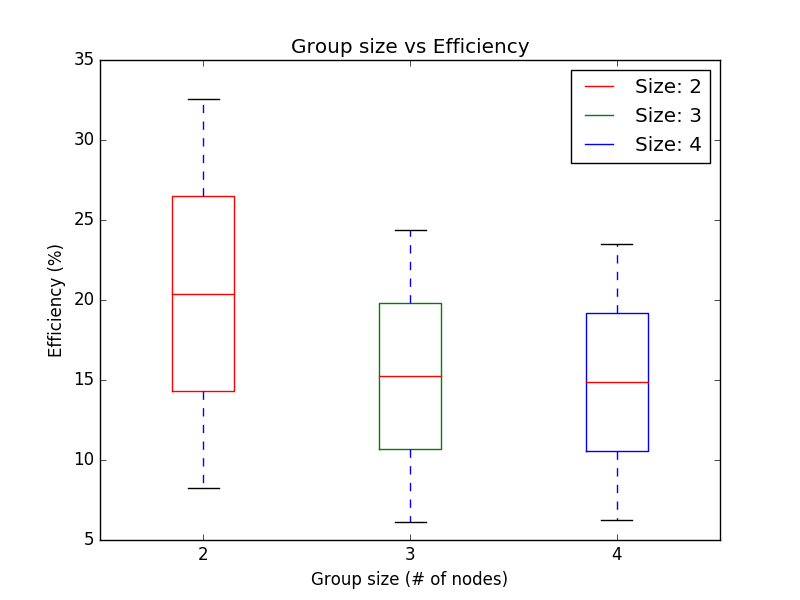
\includegraphics[scale=0.45]{GS_vs_Eff_Real.png}
   \caption{Group size vs. Efficiency within 95\% CI}
   \label{gsvseff}
\end{figure}

As for the efficiency analysis, observing its relationship with group size parameter, Figure \ref{gsvseff}, we can claim that sparser connections (i.e. smaller group sizes), will tend to increase the efficiency across the network, which is intuitively correct. If one takes the fact that more packets being exchanged will bring a risk of congestion to the network and probably resulting in more packet losses due to timeouts into consideration, the results seen from figure is quite convincing. The corresponding means and standard deviations are $20.405 \pm 4.056$, $18.298 \pm 2.033$ and $18.403 \pm 1.700$ for group sizes 2, 3 and 4, respectively. The statistics for the number of experiments conducted and the packet count analysis is similar to the experiments of the relationship between group size and average stable delivery time.

% Lambda vs Efficiency
\begin{figure}[h]
\centering
   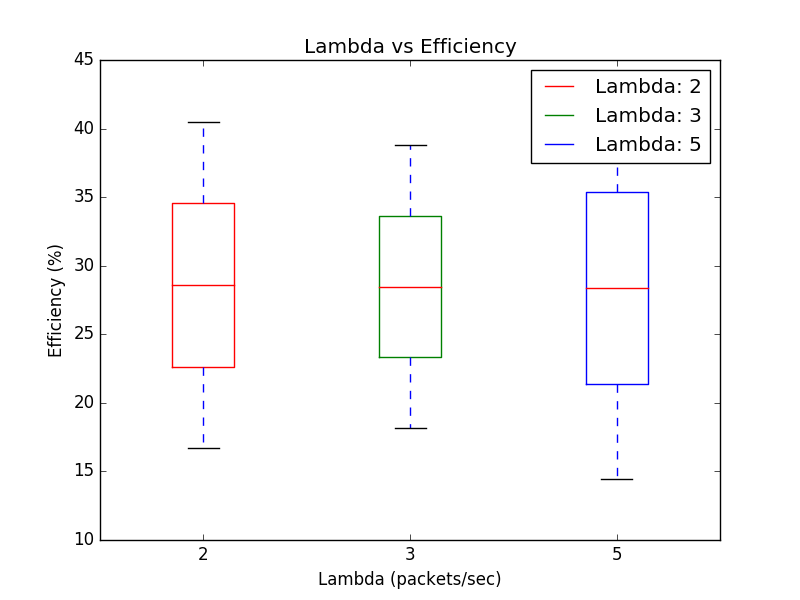
\includegraphics[scale=0.45]{Lambda_vs_Eff_Final.png}
   \caption{Lambda vs. Efficiency within 95\% CI}
   \label{lbvseff}
\end{figure}

In addition to regular group size effect, we also conducted experiments on the effect of different lambda values on the network efficiency, Figure \ref{lbvseff}. Since the group size is fixed (fixed to 2), the differences are not considerable. As it was in the lambda vs average stable delivery time experiments, the case of $\lambda = 2$ is slightly higher overall. The corresponding means and standard deviations are $28.594 \pm 3.963$, $28.480 \pm 3.443$ and $28.398 \pm 4.660$ for lambda values 2, 3 and 5, respectively. The statistics for the number of experiments conducted and the packet count analysis is similar to the experiments of the relationship between lambda and average stable delivery time.

As a final observation, one can observe that the results of average stable delivery time experiments has some negative values. Under normal circumstances, if the time synchronization was flawless and the nodes/processes ran in an order which can be converted into a sequential context, those negative values would not be visible; however, since the nodes operate asynchronously even the synchronization of global time fails within the context switches and several delays in the network. Briefly, those negative values are caused by the unsynchronized state of the nodes in the network.

\begin{thebibliography}{99}

\bibitem{CMB}
    Chandy, K. M., and J. Misra. 1981. "Asynchronous Distributed Simulation Via a Sequence of Parallel Computations." Communications of the ACM 24 (4):198-205.

\bibitem{FastCast}
    Coelho, P. R., Schiper, N., Pedone, F., "Fast Atomic Multicast", USI Technical Report Series in Informatics, 2017.

\end{thebibliography}

\end{document}
